
\documentclass[a4paper,11pt]{article}
\usepackage[a4paper, margin=8em]{geometry}

% usa i pacchetti per la scrittura in italiano
\usepackage[french,italian]{babel}
\usepackage[T1]{fontenc}
\usepackage[utf8]{inputenc}
\frenchspacing 

% usa i pacchetti per la formattazione matematica
\usepackage{amsmath, amssymb, amsthm, amsfonts}

% usa altri pacchetti
\usepackage{gensymb}
\usepackage{hyperref}
\usepackage{standalone}

% imposta il titolo
\title{Appunti Elettronica Digitale}
\author{Luca Seggiani}
\date{2026}

% imposta lo stile
% usa helvetica
\usepackage[scaled]{helvet}
% usa palatino
\usepackage{palatino}
% usa un font monospazio guardabile
\usepackage{lmodern}

\renewcommand{\rmdefault}{ppl}
\renewcommand{\sfdefault}{phv}
\renewcommand{\ttdefault}{lmtt}

% disponi il titolo
\makeatletter
\renewcommand{\maketitle} {
	\begin{center} 
		\begin{minipage}[t]{.8\textwidth}
			\textsf{\huge\bfseries \@title} 
		\end{minipage}%
		\begin{minipage}[t]{.2\textwidth}
			\raggedleft \vspace{-1.65em}
			\textsf{\small \@author} \vfill
			\textsf{\small \@date}
		\end{minipage}
		\par
	\end{center}

	\thispagestyle{empty}
	\pagestyle{fancy}
}
\makeatother

% disponi teoremi
\usepackage{tcolorbox}
\newtcolorbox[auto counter, number within=section]{theorem}[2][]{%
	colback=blue!10, 
	colframe=blue!40!black, 
	sharp corners=northwest,
	fonttitle=\sffamily\bfseries, 
	title=~\thetcbcounter: #2, 
	#1
}

% disponi definizioni
\newtcolorbox[auto counter, number within=section]{definition}[2][]{%
	colback=red!10,
	colframe=red!40!black,
	sharp corners=northwest,
	fonttitle=\sffamily\bfseries,
	title=~\thetcbcounter: #2,
	#1
}

% U.D.M
\newcommand{\amp}{\ensuremath{\mathrm{A}}}
\newcommand{\volt}{\ensuremath{\mathrm{V}}}
\newcommand{\meter}{\ensuremath{\mathrm{m}}}
\newcommand{\second}{\ensuremath{\mathrm{s}}}
\newcommand{\farad}{\ensuremath{\mathrm{F}}}
\newcommand{\henry}{\ensuremath{\mathrm{H}}}
\newcommand{\siemens}{\ensuremath{\mathrm{S}}}

% circuiti
\usepackage{circuitikz}
\usetikzlibrary{babel}

% disegni
\usepackage{pgfplots}
\pgfplotsset{width=10cm,compat=1.9}

% disponi codice
\usepackage{listings}
\usepackage[table]{xcolor}

\definecolor{codegreen}{rgb}{0,0.6,0}
\definecolor{codegray}{rgb}{0.5,0.5,0.5}
\definecolor{codepurple}{rgb}{0.58,0,0.82}
\definecolor{backcolour}{rgb}{0.95,0.95,0.92}

\lstdefinestyle{codestyle}{
		backgroundcolor=\color{black!5}, 
		commentstyle=\color{codegreen},
		keywordstyle=\bfseries\color{magenta},
		numberstyle=\sffamily\tiny\color{black!60},
		stringstyle=\color{green!50!black},
		basicstyle=\ttfamily\footnotesize,
		breakatwhitespace=false,         
		breaklines=true,                 
		captionpos=b,                    
		keepspaces=true,                 
		numbers=left,                    
		numbersep=5pt,                  
		showspaces=false,                
		showstringspaces=false,
		showtabs=false,                  
		tabsize=2
}

\lstdefinestyle{shellstyle}{
		backgroundcolor=\color{black!5}, 
		basicstyle=\ttfamily\footnotesize\color{black}, 
		commentstyle=\color{black}, 
		keywordstyle=\color{black},
		numberstyle=\color{black!5},
		stringstyle=\color{black}, 
		showspaces=false,
		showstringspaces=false, 
		showtabs=false, 
		tabsize=2, 
		numbers=none, 
		breaklines=true
}

\lstdefinelanguage{javascript}{
	keywords={typeof, new, true, false, catch, function, return, null, catch, switch, var, if, in, while, do, else, case, break},
	keywordstyle=\color{blue}\bfseries,
	ndkeywords={class, export, boolean, throw, implements, import, this},
	ndkeywordstyle=\color{darkgray}\bfseries,
	identifierstyle=\color{black},
	sensitive=false,
	comment=[l]{//},
	morecomment=[s]{/*}{*/},
	commentstyle=\color{purple}\ttfamily,
	stringstyle=\color{red}\ttfamily,
	morestring=[b]',
	morestring=[b]"
}

% disponi sezioni
\usepackage{titlesec}

\titleformat{\section}
	{\sffamily\Large\bfseries} 
	{\thesection}{1em}{} 
\titleformat{\subsection}
	{\sffamily\large\bfseries}   
	{\thesubsection}{1em}{} 
\titleformat{\subsubsection}
	{\sffamily\normalsize\bfseries} 
	{\thesubsubsection}{1em}{}

% disponi alberi
\usepackage{forest}

\forestset{
	rectstyle/.style={
		for tree={rectangle,draw,font=\large\sffamily}
	},
	roundstyle/.style={
		for tree={circle,draw,font=\large}
	}
}

% disponi algoritmi
\usepackage{algorithm}
\usepackage{algorithmic}
\makeatletter
\renewcommand{\ALG@name}{Algoritmo}
\makeatother

% disponi numeri di pagina
\usepackage{fancyhdr}
\fancyhf{} 
\fancyfoot[L]{\sffamily{\thepage}}

\makeatletter
\fancyhead[L]{\raisebox{1ex}[0pt][0pt]{\sffamily{\@title \ \@date}}} 
\fancyhead[R]{\raisebox{1ex}[0pt][0pt]{\sffamily{\@author}}}
\makeatother

\begin{document}
% sezione (data)
\section{Lezione del 10-03-26}

% stili pagina
\thispagestyle{empty}
\pagestyle{fancy}

% testo
\subsection{Giunzione P/N}
Fenomeni elettrici interessanti accadono quando si collegano 2 materiali semiconduttori (silicio) drogati con un processo rispettivamente di tipo P e di tipo N.

Supponiamo quindi dia avere un corpo rettangolare diviso in due regioni (una di tipo P e una di tipo N), collegato ad un anodo $A$ dal lato P e ad un catodo $K$ dal lato N.

\begin{itemize}
	\item 
Ricordiamo che il silicio di tipo P è un silicio drogato con atomi accettori di elettroni (quindi del terzo gruppo, ad esempio boro). Immaginiamo in questo caso di avere una concentrazione di $N_A = 10^{17} \, \mathrm{cm}^{-3}$ atomi accettori:
$$
p_P = N_A = 10^{17} \, \mathrm{cm}^{-3}, \quad n_P = \frac{n_i^2}{N_A} = \frac{10^{20}}{10^{17}} = 10^3 \, \mathrm{cm}^{-3}
$$
	\item 
Il silicio di tipo N è invece un silicio drogato con atomi donatori di elettroni (quindi del quinto gruppo, ad esempio fosforo o arsenico). Immaginiamo in questo caso di avere una concentrazione di $N_D = 10^{16} \, \mathrm{cm}^{-3}$ atomi donatori:
$$
n_N = N_D = 10^{16} \, \mathrm{cm}^{-3}, \quad p_N = \frac{n_i^2}{N_D} = \frac{10^{20}}{10^{16}} = 10^4 \, \mathrm{cm}^{-3}
$$
\end{itemize}

\begin{center}
	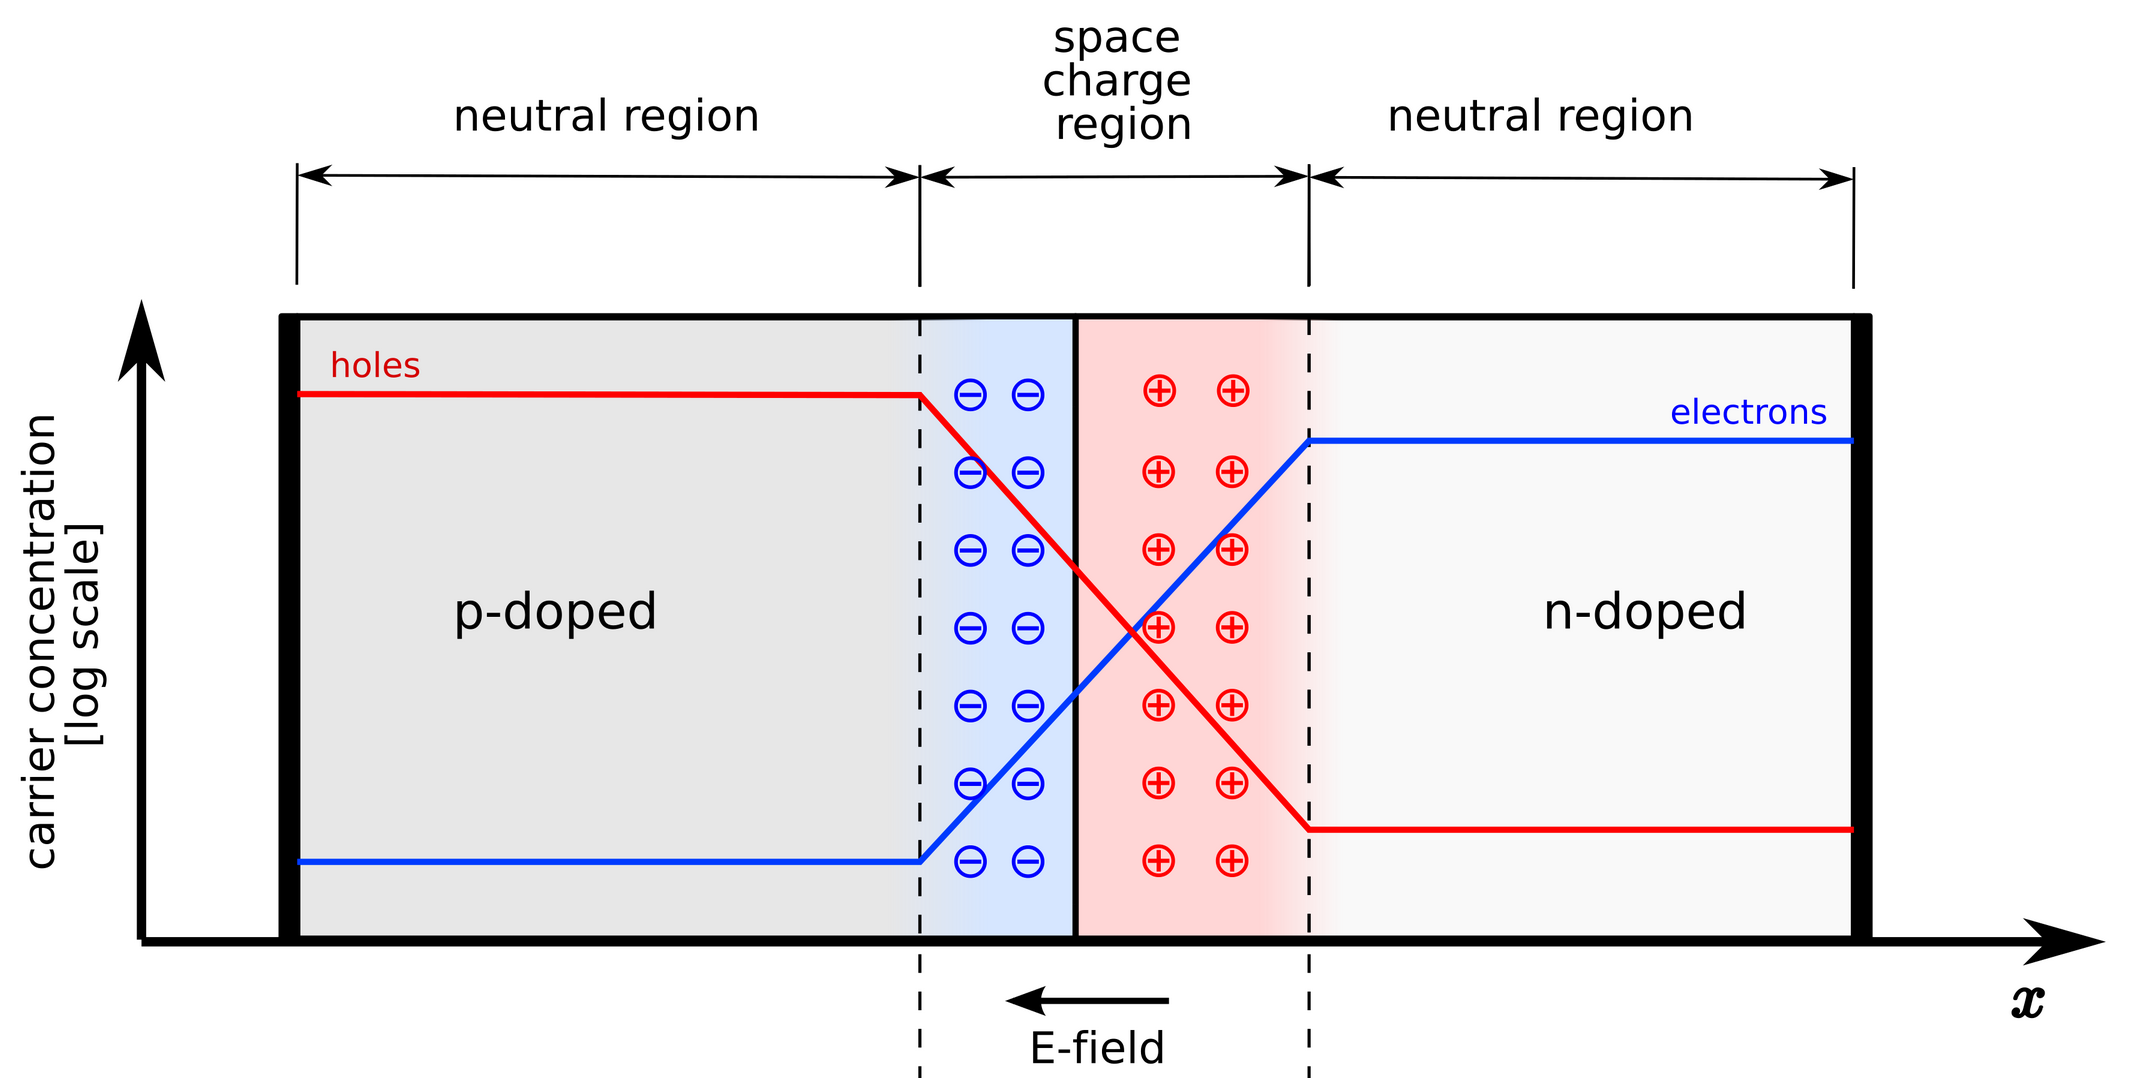
\includegraphics[scale=0.16]{../figures/pn_junct.png}
\end{center}

In questo caso abbiamo che le concentrazioni $p$ e $n$ di lacune ed elettroni liberi rispettivamente variano lungo l'asse $x$ del corpo, ed hanno un punto di incrocio nel punto centrale (chiamiamolo $\phi$). La corrente totale $\vec{I}$ che passa nel punto $\phi$ sarà quindi nulla, come lo sarà la densità di corrente $\vec{J}$.

\par\smallskip

\noindent
\textbf{\textsf{Corrente di diffusione}}

\noindent
Ciò che accadrà in una configurazione di questo tipo è però che le lacune si sposteranno da sinistra verso destra (in quanto c'è una maggiore concentrazione di lacune piuttosto che di elettroni liberi, $10^{17} > 10^{16}$).
\begin{itemize}
	\item Avevamo da 4.2 la legge di Fick della diffusione, per cui la densità di corrente di diffusione delle lacune sarà:
$$
\vec{J}_{P, \text{Diffusione}} = - e D_P \frac{\partial p}{\partial x} \hat{i}_x 
$$
	\item Allo stesso modo, la corrente di diffusione degli elettroni liberi sarà:
$$
\vec{J}_{N, \text{Diffusione}} = + e D_N \frac{\partial n}{\partial x} \hat{i}_x 
$$
\end{itemize}

Da quanto detto rispetto alla maggiore concentrazione di lacune piuttosto che di elettroni liberi, si avrà per forza che:
$$
\vec{J}_{P, \text{Diffusione}} + \vec{J}_{N, \text{Diffusione}} \neq 0
$$

Questo è apprentemente assurdo, in quanto avevamo imposto $\vec{J} = 0$. Dovrà quindi esistere una corrente di deriva che va a bilanciare le correnti di diffusione.

\par\smallskip

\noindent
\textbf{\textsf{Corrente di deriva}}

\noindent
Perchè esista una corrente di deriva deve esistere un campo elettrico. Ciò che accade è quindi che si va a formare un campo elettrico $\vec{E}$ interno alla giunzione, che forma le correnti di deriva che bilanciano le correnti di diffusione (in modo che nel complessivo si obbedisca a $\vec{J} = 0$).

Ingrandiamo quindi la zona della giunzione fra P ed N.
\begin{itemize}
	\item Nella regione P avremo una serie di ioni \textit{accettori} fissi. In condizioni di equilibrio (quindi prima di collegare la regione N), ad ognuno di questi sarà associata una lacuna libera di drogaggio, per cui la carica complessiva sarà neutra;
	\item Allo stesso modo nella regione N avremo una serie di ioni \textit{donatori} fissi. In condizioni di equilibrio (quindi prima di collegare la regione P), ad ognuno di questi sarà associato un elettrone libero di drogaggio, per cui la carica complessiva sarà anche qui neutra.
\end{itemize}

Nel momento in cui si va a formare la giunzione, avremo che le lacune nella regione P vengono a spostarsi nella regione N ed a ricombinarsi con gli elettroni liberi (in verità sono gli ioni di silicio negativi che forniscono elettroni agli ioni di silicio positivi della regione P, ma continuiamo a considerare le lacune come particelle). Allo stesso modo, gli elettroni liberi nella regione N a spostarsi nella regione P ed a ricombinarsi con le lacune libere. 

Questo processo si svolge a livello di atomi di silicio: gli ioni fissi (accettori e donatori rispettivamente nelle regioni P ed N) resteranno tali, ma la loro carica non sarà più bilanciata, per cui si genereranno 2 regioni con carica non neutra. In particolare:
\begin{itemize}
	\item Nella regione P, a maggioranza di ioni \textit{accettori} fissi, resteranno questi (carichi negativamente) e quindi si avrà carica \textit{negativa};
	\item Nella regione N, a maggioranza di ioni \textit{donatori} fissi, resteranno questi (carichi positivamente) e quindi si avrà carica \textit{positiva}.
\end{itemize}

\par\smallskip

\noindent
\textbf{\textsf{Zona di svuotamento}}

\noindent
Indichiamo con $w$ la lunghezza della combinazione delle 2 regioni così formate. Chiamiamo tale regione \textbf{zona di svuotamento}. All'interno della zona di svuotamento si andrà a formare un campo $\vec{E}$. Da quanto abbiamo detto riguardo alla corrente complessiva e alle correnti di diffusione, dovrà essere che la situazione di \textit{equilibrio} del campo $\vec{E}$ è quella che porta alla formazione di correnti di deriva bilanciano tali correnti di diffusione. In simboli si parte dal dire:
$$
\vec{J} = \vec{J}_P + \vec{J}_N = 0 \implies
\begin{cases}
	\vec{J}_P = 0 \\
	\vec{J}_N = 0 \\
\end{cases}
$$
Questo in quanto non si può avere accumulazione di lacune nella regione $N$ (che è quello che accadrebbe con $\vec{J}_P > 0$), e allo stesso modo non si può avere accumulazione di elettroni nella regione $P$ (che è quello che accadrebbe con $\vec{J}_N > 0$). Resta che l'unica possibilità è che siano entrambe 0.

Possiamo quindi porre separatamente:
$$
\begin{cases}
	\vec{J}_N = + e D_N \frac{\partial n}{\partial x} \hat{i}_x + n e \mu_N \vec{E} = 0 \\
	\vec{J}_P = - e D_P \frac{\partial p}{\partial x} \hat{i}_x + p e \mu_P \vec{E} = 0
\end{cases}
$$
e quindi risolvere le 2 equazioni ottenute per ottenere 2 equazioni (entrambe valide) per il campo che si va a formare nella zona di svuotamento:
$$
\begin{cases}
	E = -\frac{D_n}{n \mu_n} \frac{dn}{dx} \\ 
	E = +\frac{D_è}{n \mu_p} \frac{dp}{dx}
\end{cases}
$$
dove ci siamo riportati a scalari prendendo tutti i vettori paralleli. Possiamo quindi prendere la legge di Einstein delle costanti di diffusione vista a 4.3, che in particolare diceva:
$$
\frac{D_n}{\mu_n} = \frac{D_p}{\mu_p} = \frac{k_B T}{e}
$$
Usiamo tale stima per esprimere diversamente i rapporti costante di diffusione / mobilità:
$$
\begin{cases}
	E = -\frac{k_B T}{e} \frac{1}{n} \frac{dn}{dx} \\ 
	E = +\frac{k_B T}{e} \frac{1}{p} \frac{dp}{dx} 
\end{cases}
$$
che è la formula del campo all'interno della zona di svuotamento. Vedremo come queste definizioni ci torneranno utili a breve, nel calcolo della \textit{barriera di tensione}.

\par\smallskip

\noindent
\textbf{\textsf{Descrizione qualitativa del campo}}

\noindent
\begin{center}
	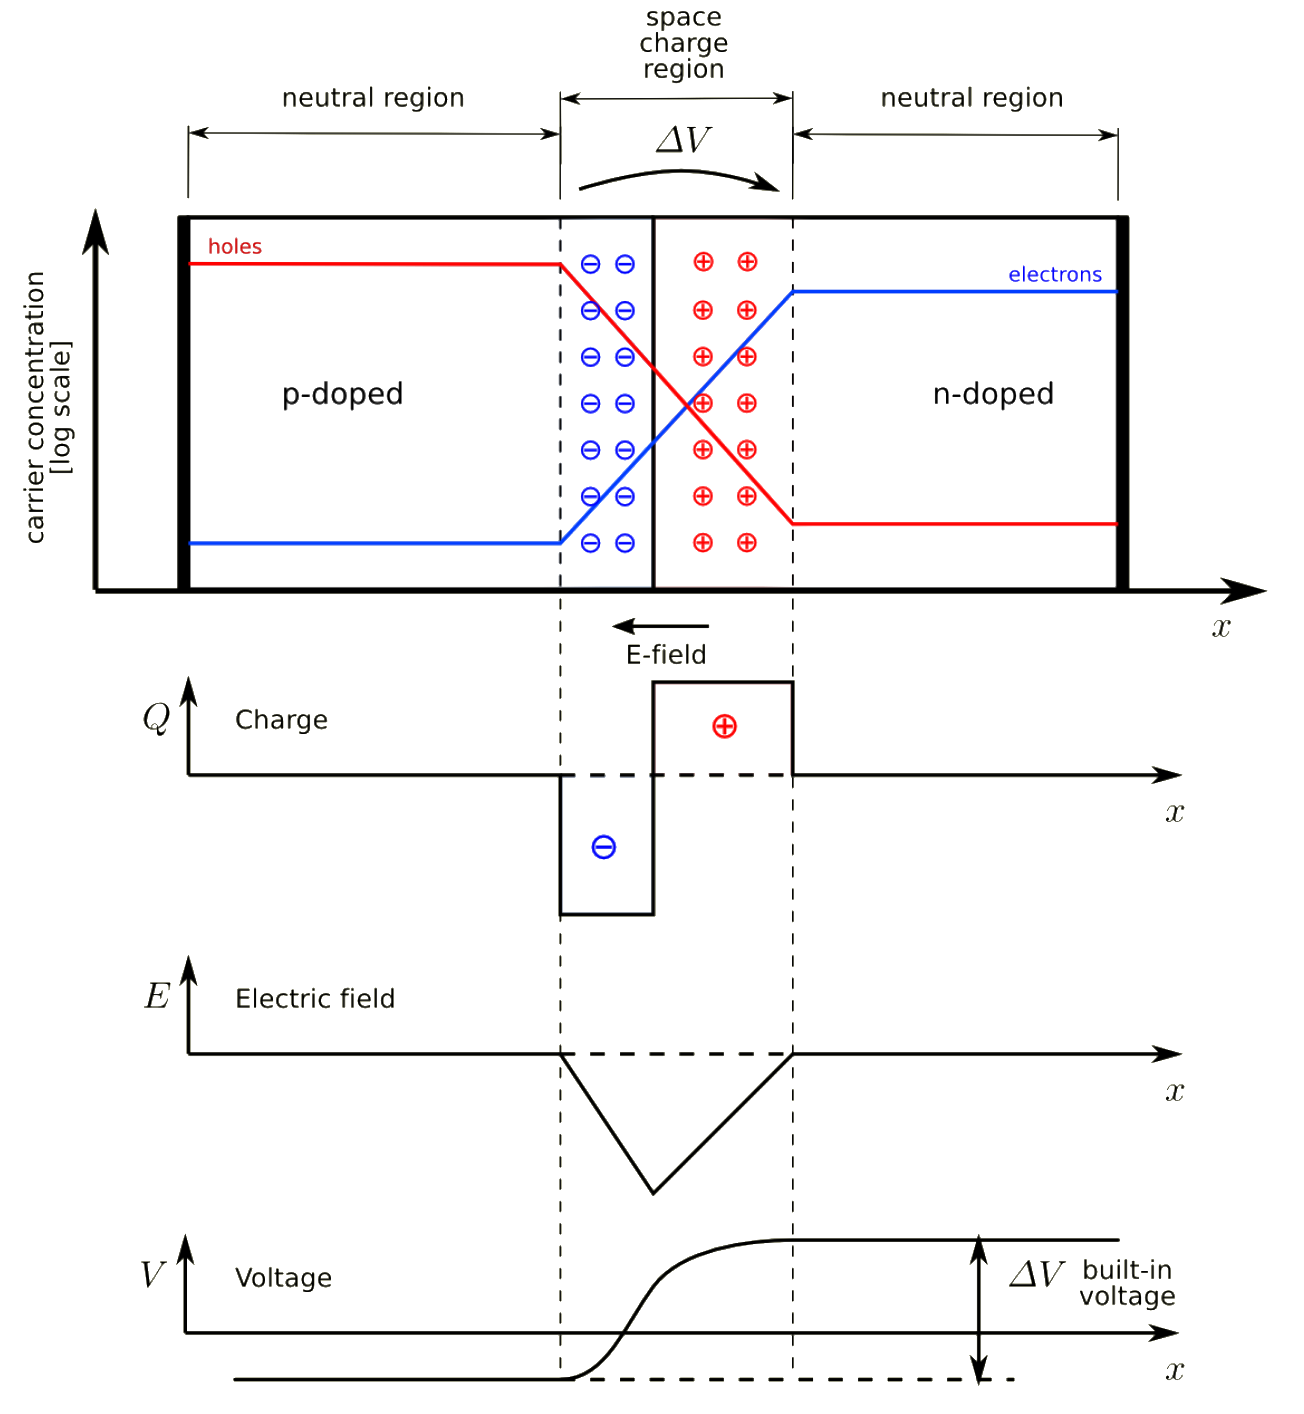
\includegraphics[scale=0.26]{../figures/pn_junct_field.png}
\end{center}

Vediamo quindi la descrizione qualitativa del campo che si va a formare. Prima di tutto, abbiamo che nella zona di svuotamento si avranno una prima regione negativa e quindi una regione positiva (chiamiamo $Q(x)$ la funzione di carica). Se l'equilibrio è rispettato, dovra essere che l'integrale della carica nella zona negativa dovrà essere uguale a quello nella zona positiva. Questo va specificato in quanto, visto che le lacune sono più degli elettroni, si ha che la barriera $\phi$ fra le due regione è leggermente spostata verso la regione P. 

Una volta nota la carica $Q(x)$, possiamo calcolare il campo $E(x)$ applicando la definizione come:
$$
\frac{d E(x)}{dx} = -\frac{Q(x)}{S \epsilon_0}
$$
dove $S$ è la sezione della giunzione e $\epsilon_0$ è la permittività dello spazio. Come vediamo, questo significherà che abbiamo un picco di campo elettrico $\vec{E}$ (negativo, dalla zona N alla zona P) nel punto $\phi$. Ai limiti della zona di svuotamento andranno considerati gli opportuni effetti di bordo.

\par\smallskip

\noindent
\textbf{\textsf{Barriera di potenziale}}

\noindent
Infine, possiamo interrogarci riguardo al potenziale $V(x)$. In generale, vale:
$$
E(x) = -\frac{d V(x)}{dx}
$$
Questo, nella giunzione appena vista, implica la seguente legge:
\begin{theorem}{Barriera di potenziale}
In una giunzione P/N, per via del campo $E$ che si forma nella zona di svuotamento, si avrà la formazione di un campo $V_0$.
$$
\Delta V = V_0 = \frac{k_B T}{q} \ln \left( \frac{N_A N_D}{n_i^2} \right)
$$
\end{theorem}

Chiamiamo questa differenza di potenziale $\Delta V$ che si misura fra la regione prossima all'anodo e la regione prossima al catodo della giunzione \textbf{potenziale "built-in"} interno alla giunzione.

Il calcolo di $\Delta V$ è banale note le espressioni del campo $E$ viste 2 sezioni fa. Possiamo procedere usando l'espressione sia in funzione dei portatori negativi $n$ che in funzione dei portatori positivi $p$.

\begin{itemize}
	\item Se si sceglie di preseguire con i portatori $n$, si ha l'espressione del campo:
$$
E = -\frac{k_B T}{e} \frac{1}{n} \frac{dn}{dx} 
$$
dalla definizione del potenziale si ottiene di dover integrare:
$$
E = -\frac{dV}{dx} \implies V = - \int^{N_D}_\frac{n_i^2}{N_A} E \, dx =  \int^{N_D}_\frac{n_i^2}{N_A} \frac{k_B T}{e} \frac{1}{n} \frac{dn}{\not{dx}} \, \not{dx}
$$
Soffermiamoci un istante sugli estremi di integrazione. Abbiamo che finiamo per integrare su $dn$, per cui dobbiamo prendere la variazione di $n$ sul percorso dove calcoliamo il potenziale, cioè dall'estremo $N$ all'estremo $P$ della giunzione.
\begin{itemize}
	\item All'estremo $N$ della giunzione si ha che, per il doping di tipo N, la densità elettronica è semplicemente:
		$$
		n = N_D
		$$
	\item All'estremo $P$ della giunzione si ha che, per il doping di tipo P e la legge massa-azione (4.1), la densità elettronica è:
		$$
		n = \frac{n_i^2}{N_A}
		$$
\end{itemize}
da cui gli estremi che vediamo nell'integrale. Risolvendo si ottiene quindi:
$$
V = \int^{N_D}_\frac{n_i^2}{N_A} \frac{k_B T}{e} \frac{1}{n} \, dn = \frac{k_B T}{e} \ln(n) \Big|^{N_D}_\frac{n_i^2}{N_A} =  \frac{k_B T}{q} \ln \left( \frac{N_A N_D}{n_i^2} \right)
$$
che è quanto stavamo cercando.

\item Il processo con i portatori $p$ è analogo, si ha l'espressione del campo:
$$
E = +\frac{k_B T}{e} \frac{1}{p} \frac{dp}{dx} 
$$
e l'integrale è:
$$
V = - \int^\frac{n_i^2}{N_D}_{N_A} E \, dx = - \int^\frac{n_i^2}{N_D}_{N_A} \frac{k_B T}{e} \frac{1}{p} \frac{dp}{\not{dx}} \, \not{dx}
$$
Gli estremi di integrazione sono scelti come prima. Abbiamo che finiamo per integrare su $dp$, per cui dobbiamo prendere la variazione di $p$ sul percorso dove calcoliamo il potenziale, cioè dall'estremo $N$ all'estremo $P$ della giunzione.
\begin{itemize}
	\item All'estremo $N$ della giunzione si ha che, per il doping di tipo N e la legge massa-azione, la densità di lacuna è:
		$$
		n = \frac{n_i^2}{N_D}
		$$
	\item All'estremo $P$ della giunzione si ha che, per il doping di tipo P, la densità di lacuna è semplicemente:
		$$
		p = N_A
		$$
\end{itemize}
da cui gli estremi che vediamo nell'integrale. Risolvendo si ottiene quindi:
$$
V = - \int^\frac{n_i^2}{N_D}_{N_A} \frac{k_B T}{e} \frac{1}{p} \, dp = \frac{k_B T}{e} \ln(p) \Big|^\frac{n_i^2}{N_D}_{N_A} =  \frac{k_B T}{q} \ln \left( \frac{N_A N_D}{n_i^2} \right)
$$
che è nuovamente quanto stavamo cercando.

\end{itemize}

In verità, fra l'anodo e la giunzione con la regione P si viene a formare un \textbf{potenziale di contatto} $V_1$, e allo stesso modo fra il catodo e la giunzione con la regione N si viene a formare un'altro potenziale di contatto $V_2$. Si dimostra che:
$$
V_1 + V_2 + V_0 = 0
$$
per cui è impossibile misurare direttamente il potenziale built-in $\Delta V$ a partire da anodo e catodo. Notiamo però che tale potenziale esiste comunque all'interno della giunzione. 

Notiamo quindi che nel complesso:
\begin{itemize}
	\item Una lacuna che vuole spostarsi dalla regione P alla regione N deve vincere il potenziale "built-in" $\Delta V$. Questo perché l'energia potenziale di lacuna è:
		$$
			U = q V
		$$
		e spostarsi da sinistra verso destra significa aumentare $V$, quindi aumentare propria energia potenziale;
	\item Un elettrone libero che vuole spostarsi dalla regione N alla regione P deve vincere sempre lo stesso potenziale "built-in" $\Delta V$. Questo perché l'energia potenziale elettronica è:
		$$
			U = -q V
		$$
		e spostarsi da destra verso sinistra significa diminuire $V$, quindi aumentare la propria energia potenziale;
\end{itemize}

Si ha quindi che il potenziale "built-in" funge in qualche modo da \textit{barriera di potenziale} per la corrente che viaggia da sinistra verso destra lungo la giunzione.

\par\smallskip

\noindent
\textbf{\textsf{Bias in avanti}}

\noindent
Vediamo cosa accade quando si collega la giunzione P/N ad un generatore di potenziale $V$ che ponga l'anodo a tensione positiva e il catodo a tensione negativa. Si dice in questo caso che si dà un \textbf{bias in avanti} alla giunzione.

\begin{center}
	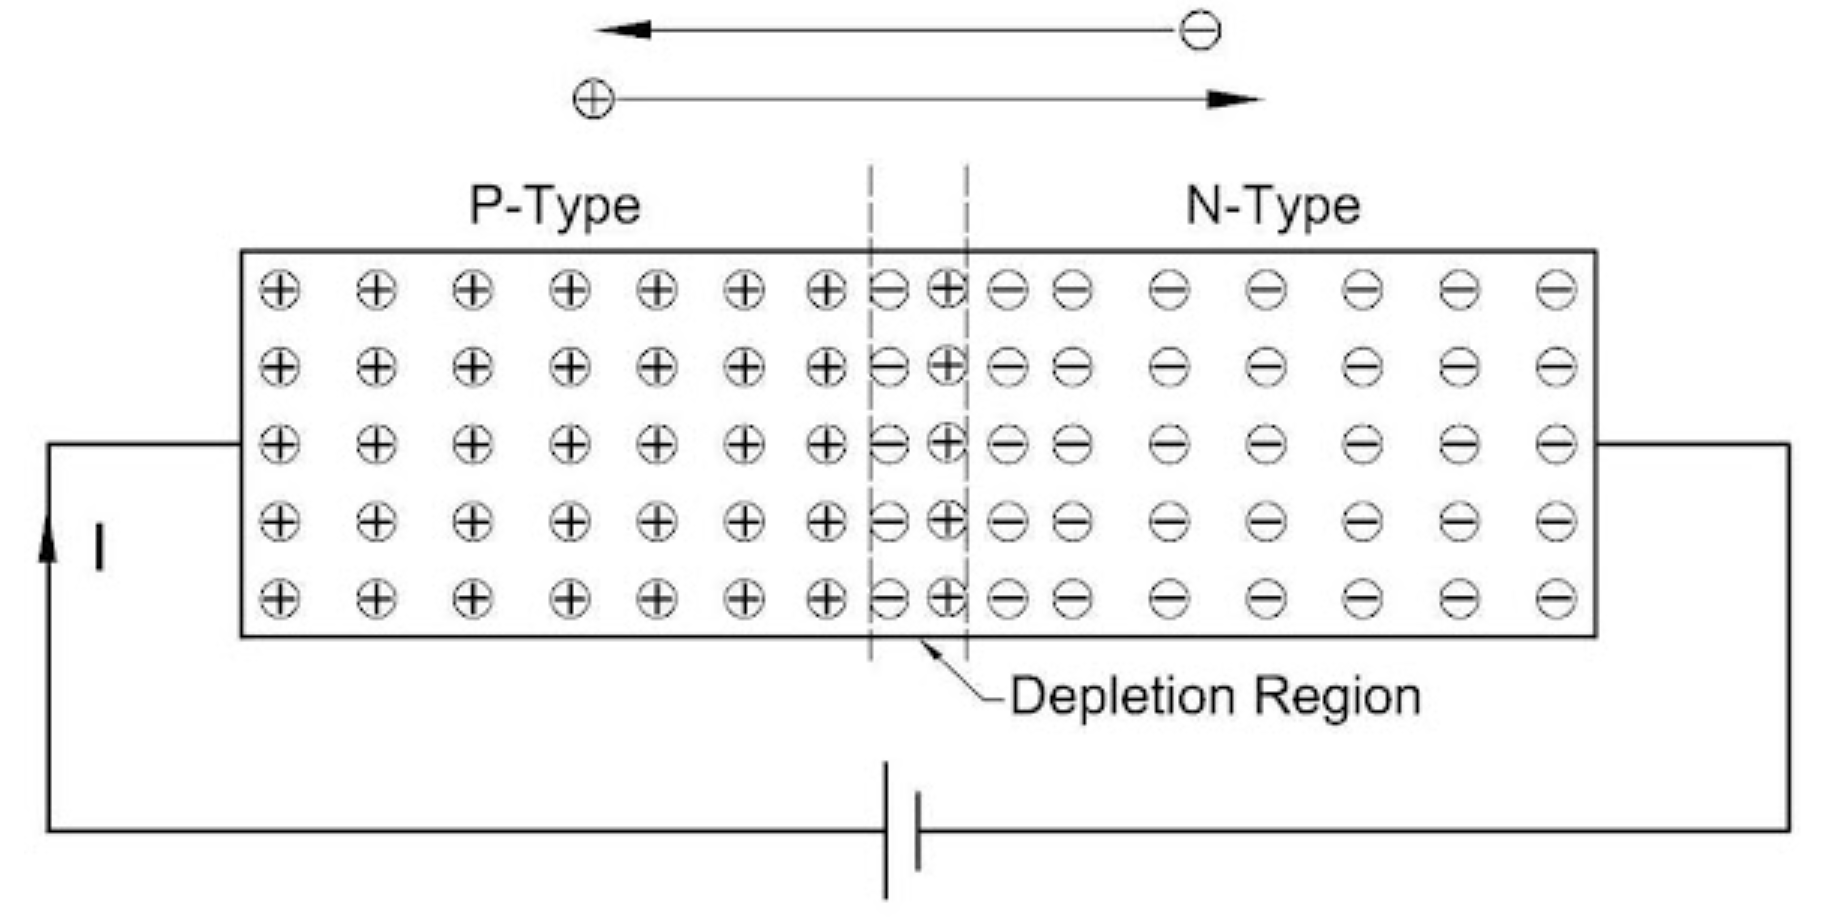
\includegraphics[scale=0.2]{../figures/forward_bias.png}
\end{center}

Il primo effetto che osserviamo è che la barriera di potenziale diminuisce, in quanto introduciamo un nuovo potenziale $V$ che va a diminuire $\Delta V$:
$$
\Delta V = V_0 - V
$$

Questo avrà un effetto sulle correnti di diffusione e di deriva che hanno luogo all'interno della zona di svuotamento della giunzione. In particolare:
\begin{itemize}
	\item Le densità di corrente di \textit{diffusione} $\vec{J}_{N, \text{Diffusione}}$ e $\vec{J}_{P, \text{Diffusione}}$ aumenteranno in quanto sarà ridotta la barriera di potenziale che gli elettroni e le lacune rispettivamente dovranno vincere;
	\item Per quanto riguarda le densità di corrente di \textit{deriva} $\vec{J}_{N, \text{Drift}}$ e $\vec{J}_{P, \text{Drift}}$, invece si avrà che queste sono piccole e restano costanti. Questè perchè le cariche che si spostano nella zona di svuotamento per effetto del campo che vi si forma sono le cariche minoritarie di ciascuna regione:
		\begin{itemize}
			\item Per effetto del campo elettrico $E$ formato, le lacune della regione N (portatrici minoritarie) derivano verso la regione P di minore potenziale;
			\item Allo stesso modo, gli elettroni della regione P (portatori minoritari) derivano verso la regione N di maggiore potenziale.
		\end{itemize}
\end{itemize}

Visto che la corrente di diffusione aumenta esponenzialmente, si ha che la conduzione può effettivamente accadere nella regione di svuotamento, e avviene con maggioranza di corrente di diffusione (piuttosto che di drift).
Il risultato sarà che la densità di corrente complessiva $\vec{J}$ non sarà più nulla, ma invece:
$$
\vec{J} \neq 0
$$

\par\smallskip

\noindent
\textbf{\textsf{Bias all'indietro}}

\noindent
Vediamo la situazione opposta, cioè quella dove si collega la giunzione P/N ad un generatore di potenziale $V$ che ponga l'anodo a tensione negativa e il catodo a tensione positiva. Si dice in questo caso che si dà un \textbf{bias all'indietro} alla giunzione.

\begin{center}
	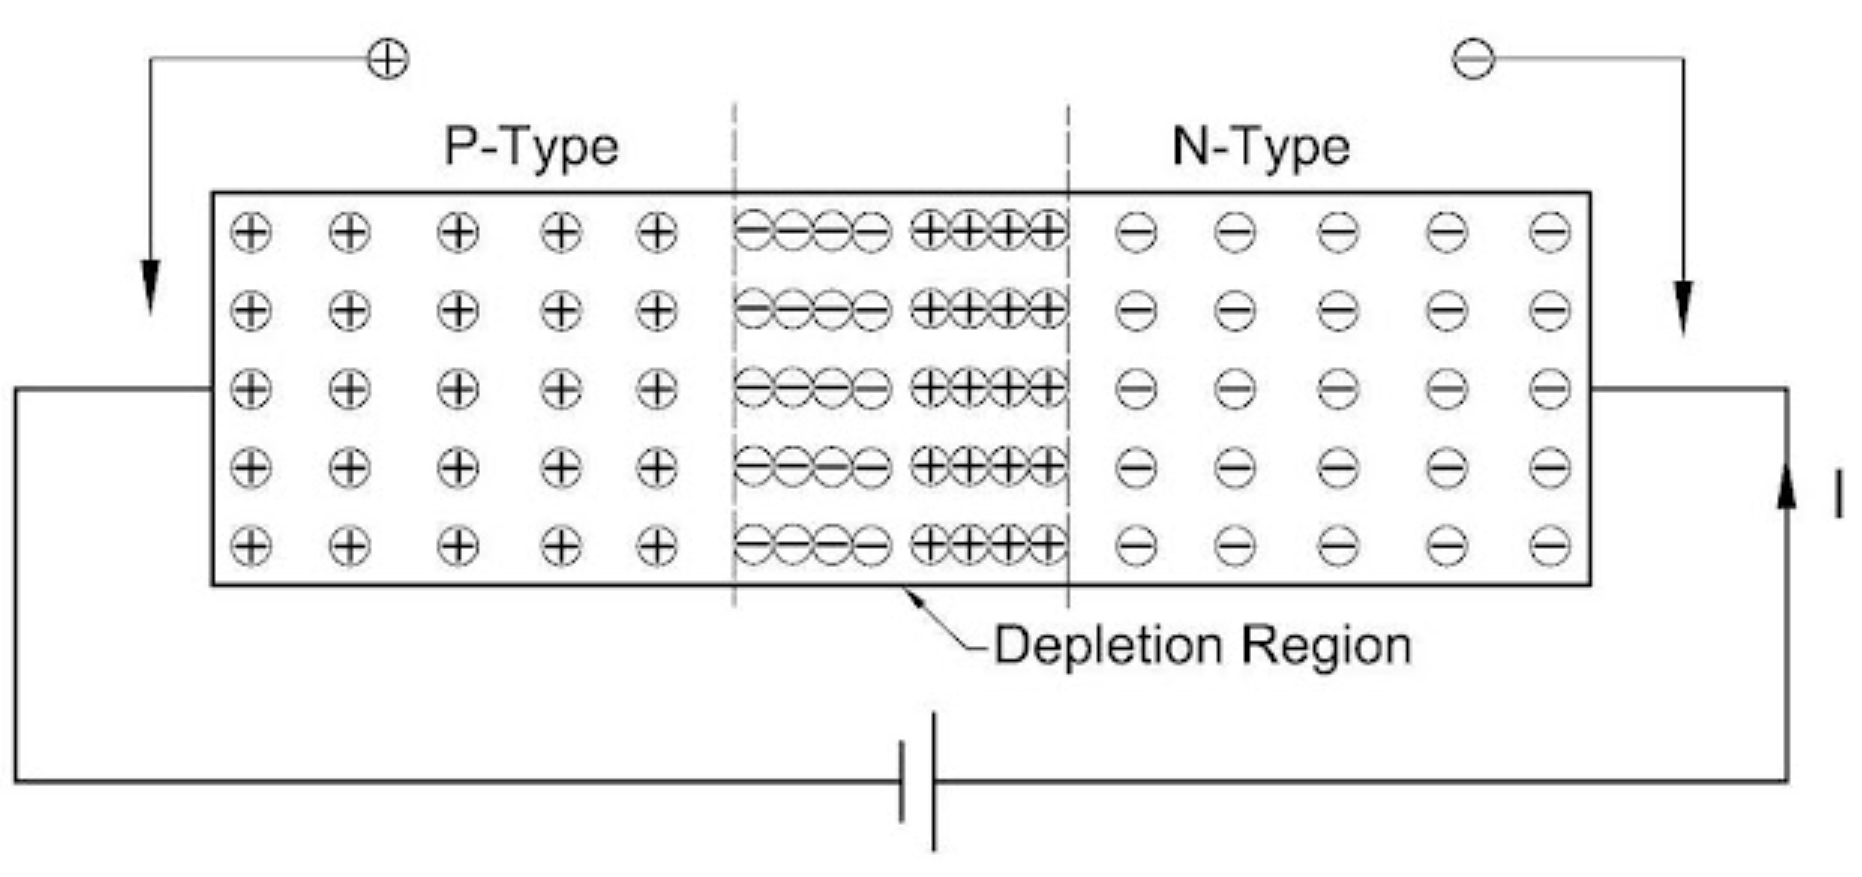
\includegraphics[scale=0.2]{../figures/reverse_bias.png}
\end{center}

Il primo effetto che osserviamo è che in questo  la barriera di potenziale aumenta, in quanto introduciamo un nuovo potenziale $V$ che va ad aumentare $\Delta V$:
$$
\Delta V = V_0 + V
$$

Come nella situazione di bias in avanti, si avrà un effetto sulle correnti di diffusione e di deriva che hanno luogo all'interno della zona di svuotamento della giunzione. In particolare:
\begin{itemize}
	\item Le densità di corrente di \textit{diffusione} $\vec{J}_{N, \text{Diffusione}}$ e $\vec{J}_{P, \text{Diffusione}}$ diminuiranno in quanto sarà aumentata la barriera di potenziale che gli elettroni e le lacune rispettivamente dovranno vincere;
	\item Per quanto riguarda le densità di corrente di \textit{deriva} $\vec{J}_{N, \text{Drift}}$ e $\vec{J}_{P, \text{Drift}}$, invece si avrà che queste sono piccole e restano costanti secondo le stesse motivazioni della scorsa sezione.
\end{itemize}

Visto che la corrente di diffusione dimunisce esponenzialmente, si ha che la conduzione può effettivamente accadere nella regione di svuotamento, e avviene con maggioranza di corrente di drift, cioè questa riesce a vincere la corrente di diffusione. 
Nuovamente si ha che la densità di corrente complessiva $\vec{J}$ non sarà più nulla, ma invece:
$$
\vec{J} \neq 0
$$
Questa densità di corrente sarà quindi dominata dal drift, e sarà \textit{piccola}, rivolta da catodo verso anodo (quindi all'opposto della corrente vista nel bias in avanti).

\par\smallskip

\noindent
\textbf{\textsf{Larghezza della zona di svuotamento}}

\noindent
Notiamo che la \textit{larghezza} della zona di svuotamento dipende dalla $V$ che imponiamo nei bias in \textit{avanti} e all'\textit{indietro}. In particolare, dipende da:
$$
w = \sqrt{ \frac{2 \epsilon_0}{q} \left( \frac{1}{N_A} + \frac{1}{N_d} \right) (V_0 - V)}
$$
Per cui:
\begin{itemize}
	\item Nel caso del bias in avanti, si ha una \textit{diminuzione} della larghezza della zona di svuotamento $w$;
	\item All'inverso, nel caso del bias all'indietro, si ha un \textit{aumento} della larghezza della zona di svuotamento $w$;
\end{itemize}

\subsubsection{Diodi}
Le giunzioni P/N come le abbiamo studiate formano quei componenti elettronici noti come \textbf{diodi}, col simbolo del componente circuitale:
\begin{center}
	\begin{circuitikz}
	\draw (0,0) to[D] (3,0);
	\end{circuitikz}
\end{center}

I diodi sono governati dalla cosiddetta legge di \textit{Shockley}:
\begin{definition}{Legge di Shockley}
La corrente $I_D$ su un diodo sottoposto a tensione $V_D$ dipende da:
$$
I_D = I_S \left( e^\frac{V_D}{\eta V_T} - 1 \right)
$$
\end{definition}
dove $I_S$ è la \textit{corrente inversa di saturazione}, $\eta$ è il \textit{fattore di idealità}, e $V_T$ è la tensione termica:
$$
V_T = \frac{k_B T}{q}
$$
già vista nella legge di Einstein a 4.3, già usata per il calcolo del potenziale "built-in" della giunzione P/N in 5.1.

\end{document}
